\chapter{Analysis}
The purpose of this chapter is to compare the SRS data structure to the kd-tree. We are going to perform a variety of tests on the SRS data structure and the kd-tree in order to determine the run-time properties of both, mainly looking at when the SRS data structure performs better than the kd-tree.


In order to compare these two data structure random data will be generated and given as input to both, such that both operate on the exact same data. When running a specific test, different data sets are generated during such that one tests is not only performed one a single data set. When the size of a slice has been determined, the search will be performed different places in the data structure such that not only best-case or worst-case scenarios occur. Finally the average of all the searches are returned as the result of the test.


\section{Vertical and horizontal slices}
The first thing to be tested is how big the vertical and horizontal slices can become before the SRS data structure performs worse than the kd-tree. We are going to look at the horizontal slices first. Below are some graphs showing the running time of a search query to both the SRS and the kd-tree dependent on the size of the slice.

Before introducing the graphs, we are going to look at the run-time of a search query to the kd-tree and the SRS data structure. A search query to the kd-tree has a run-time of $\mathcal{O}(\sqrt{n}+k)$ and a search query to the SRS data structure has a run-time of $\mathcal{O}(\lg n + k \cdot \lg^\epsilon n)$. When increasing the size of a slice, we expect the run-time of the two search queries to be roughly equal at $k \approx \frac{sqrt{n}}{lg^\epsilon n}$ stemming from $\sqrt{n} + k = \lg n + k \cdot \lg^\epsilon n \Leftrightarrows k = \frac{\sqrt{n} - \lg n}{\lg^\epsilon n - 1}$. The $\mathcal{O}(\lg^\epsilon n)$ describes the amount of jumps needed to perform in order to find the identity of a leaf given the identity of a ball in the ball inheritance structure. Thus, the size of $\mathcal{O}(\lg^\epsilon n)$ on how $B$ is chosen in \todo{ref} and which other meassures have been taken in order to lessen the amount of jumps. \todo{Skriv om at vi har målt dem også, og at de er sat ind på en graf - det er de værste hop vi kigger på? eller er det gennemsnittet? Hvad med grafen der viser $\frac{Skæringspunkt}{\frac{\sqrt{n}{lg^\epsilon n}}$ - skal det være worst $\lg^\epsilon n$ eller gennemsnittet?}

\begin{figure}[h]
    \centering
    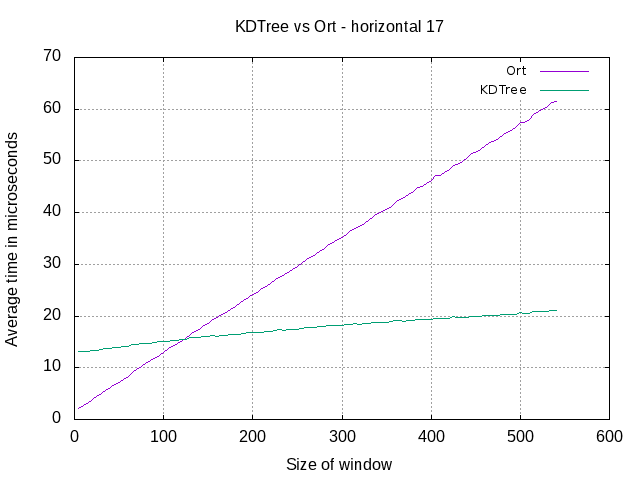
\includegraphics[width = 0.85\textwidth]{pictures/analysis/hori_17.png}
    \caption{Horizontal slice on SRS and kd-tree - data set size of $n=2^{17}$}\label{fig:hori_17}
\end{figure}


\begin{figure}[h]
    \centering
    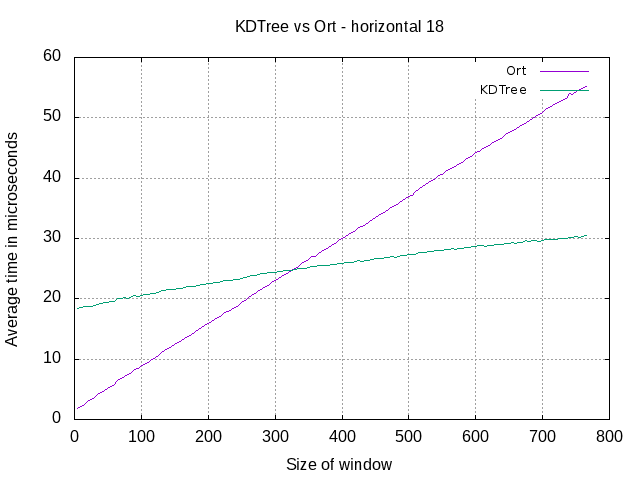
\includegraphics[width = 0.85\textwidth]{pictures/analysis/hori_18.png}
    \caption{Horizontal slice on SRS and kd-tree - data set size of $n=2^{18}$}\label{fig:hori_18}
\end{figure}


\begin{figure}[h]
    \centering
    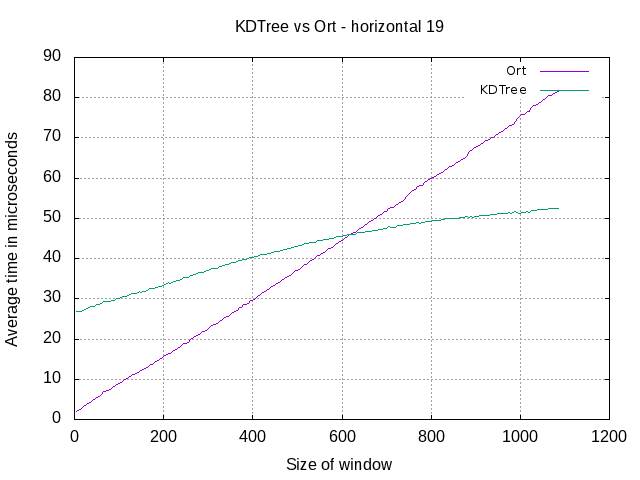
\includegraphics[width = 0.85\textwidth]{pictures/analysis/hori_19.png}
    \caption{Horizontal slice on SRS and kd-tree - data set size of $n=2^{19}$}\label{fig:hori_19}
\end{figure}


\begin{figure}[h]
    \centering
    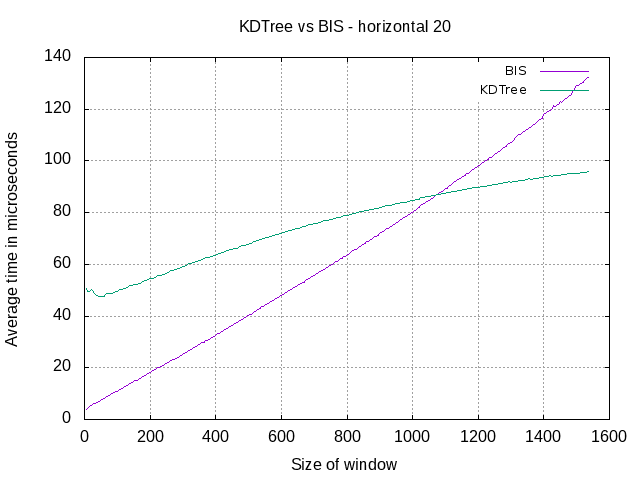
\includegraphics[width = 0.85\textwidth]{pictures/analysis/hori_20.png}
    \caption{Horizontal slice on SRS and kd-tree - data set size of $n=2^{20}$}\label{fig:hori_20}
\end{figure}


\begin{figure}[h]
    \centering
    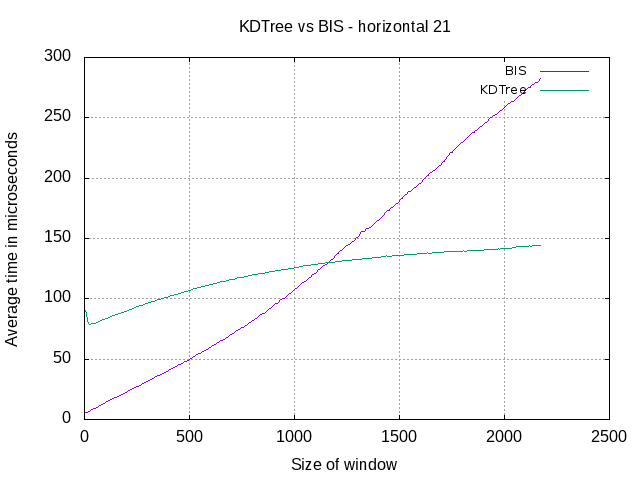
\includegraphics[width = 0.85\textwidth]{pictures/analysis/hori_21.png}
    \caption{Horizontal slice on SRS and kd-tree - data set size of $n=2^{21}$}\label{fig:hori_21}
\end{figure}

\begin{figure}[h]
    \centering
    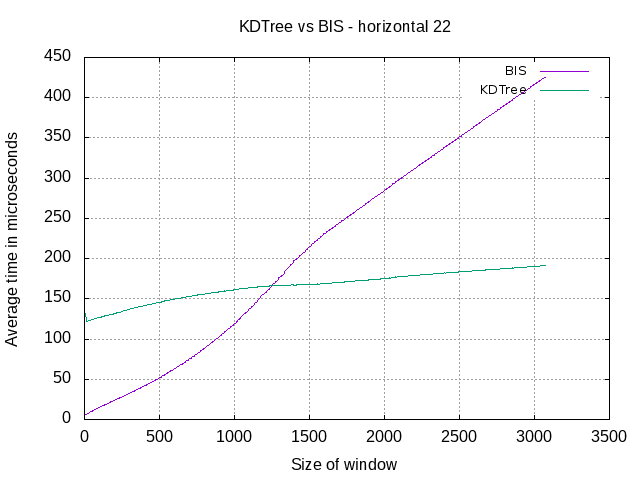
\includegraphics[width = 0.85\textwidth]{pictures/analysis/hori_22.png}
    \caption{Horizontal slice on SRS and kd-tree - data set size of $n=2^{22}$}\label{fig:hori_22}
\end{figure}

\begin{figure}[h]
    \centering
    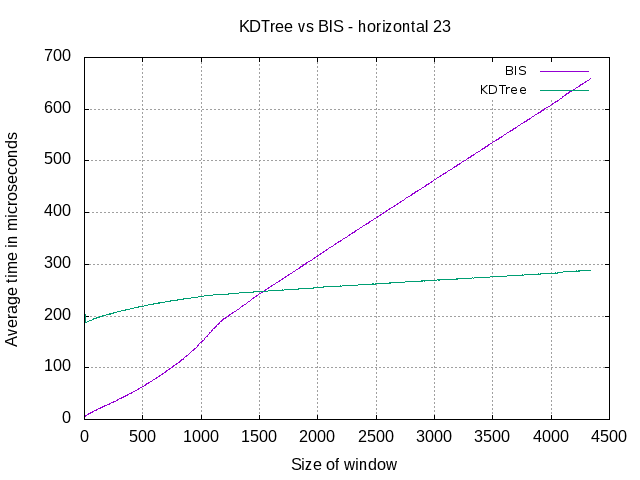
\includegraphics[width = 0.85\textwidth]{pictures/analysis/hori_23.png}
    \caption{Horizontal slice on SRS and kd-tree - data set size of $n=2^{23}$}\label{fig:hori_23}
\end{figure}

\todo{Hvorfor knækker grafen mellem $512$ og $1024$? Hvorfor er kd-træet mærkeligt dårligt inden $k=10$?}

To summarize these graphs, there is a graph of the size of the slice at the intersection between the SRS and kd-tree for each $n$ tested.

\begin{figure}[h]
    \centering
    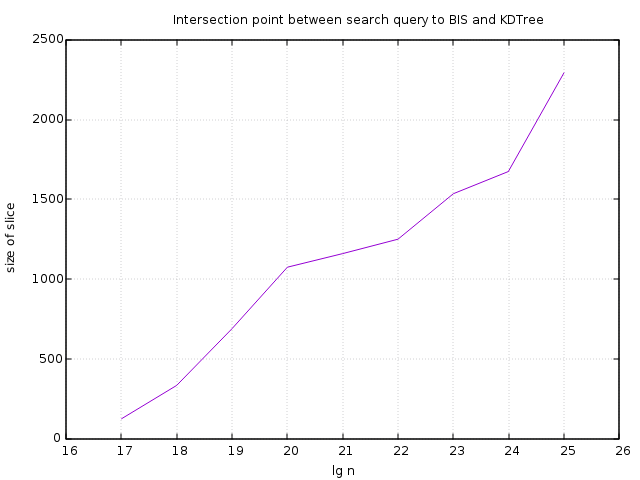
\includegraphics[width = 0.85\textwidth]{pictures/analysis/hori.png}
    \caption{Horizontal slices, intersection between running time of SRS and kd-tree}\label{fig:hori_intersection}
\end{figure}


